\chapter{Ergebnisse}
\label{chapter:results}

Das folgende Kapitel präsentiert eine eingehende Analyse der Ergebnisse, 
die aus dem linearen Regressionsmodell gewonnen wurden, welches entwickelt wurde, 
um die Runtime basierend auf verschiedenen Parametern aus dem SGEMM GPU Kernel Performance 
Datensatz zu prognostizieren. Neben der detaillierten Darstellung der Modellkoeffizienten und 
der zugehörigen Metriken umfasst dieses Kapitel auch eine Vorstellung der SHAP-Werte 
zur Interpretation der Modellvorhersagen und zur Einsicht in die Wichtigkeit der einzelnen Merkmals.

\section{Lineares Regressionmodell}

Die Koeffizienten des Modells, die in 
Tabelle \ref{tab:model-coefficients} aufgeführt sind, zeigen, wie stark sich eine 
Einheitänderung jedes unabhängigen Merkmals auf die Runtime auswirkt. 
Positive Koeffizienten deuten auf eine Erhöhung der Runtime bei Zunahme der Variablen hin, 
während negative Koeffizienten eine Verringerung anzeigen. Der Intercept-Wert repräsentiert 
die geschätzte Runtime, wenn alle unabhängigen Variablen den Wert Null annehmen. Daraus ergbit sich
zusammen mit Gleichung \ref{eq:reg-model} die Regressionsgerade für das Modell.

\begin{table}[!h]
    \centering
    \caption{Koeffizienten des linearen Regressionsmodells}
    \begin{tabularx}{\textwidth}{Xr}
    \toprule
    Merkmal ($\beta_j$) & Koeffizient \\
    \midrule
    Intercept ($\beta_0$) & 4.23287 \\
    MWG & 0.01336 \\
    NWG & 0.01057 \\
    KWG & 0.01239 \\
    MDIMC & -0.05684 \\
    NDIMC & -0.05493 \\
    MDIMA & 0.00020 \\
    NDIMB & -0.00003 \\
    KWI & -0.00422 \\
    VWM & -0.00917 \\
    VWN & -0.02371 \\
    STRM & -0.13102 \\
    STRN & -0.01729 \\
    SA & -0.18991 \\
    SB & -0.04747 \\
    \bottomrule
    \end{tabularx}
    \label{tab:model-coefficients}
\end{table}

Die Modellmetriken, dargestellt in Tabelle \ref{tab:model-metrics}, 
geben Auskunft über die Vorhersagegenauigkeit und die Anpassungsgüte des Modells. 
Der MAE und RMSE liefern dabei Informationen über die durchschnittliche Größe 
der Fehler in den Vorhersagen, und die R²-Werte zeigen, wie gut das Modell die Varianz 
der Zielvariable erklärt.

\begin{table}[!h]
    \centering
    \caption{Modellmetriken des linearen Regressionsmodells}
    \begin{tabularx}{\textwidth}{Xr}
    \toprule
    Metrik & Wert \\
    \midrule
    Mean Absolute Error (MAE) & 0.6000 \\
    Mean Squared Error (MSE) & 0.5600 \\
    Root Mean Squared Error (RMSE) & 0.7500 \\
    Training Score (R²) & 0.5622 \\
    Test Score (R²) & 0.5571 \\
    \bottomrule
    \end{tabularx}
    \label{tab:model-metrics}
\end{table}

Darüber hinaus wurden die tatsächlichen gegen die vorhergesagten Werte der Runtime
in Abbildung \ref{pic:residuals} visualisiert, die eine allgemeine Einschätzung der 
Modellgenauigkeit ermöglicht. Ein weiterer wichtiger Aspekt sind die Residuen des Modells. 
Die Residuen, also die Differenzen zwischen den tatsächlichen und vorhergesagten Werten, 
sollten idealerweise zufällig um Null verteilt sein und keine Muster aufweisen, 
die auf eine Verletzung der Modellannahmen hindeuten könnten.

\begin{figure}[!h]
    \caption{Residuenanalyse: Beziehung zwischen Vorhersagen und Abweichungen.}
    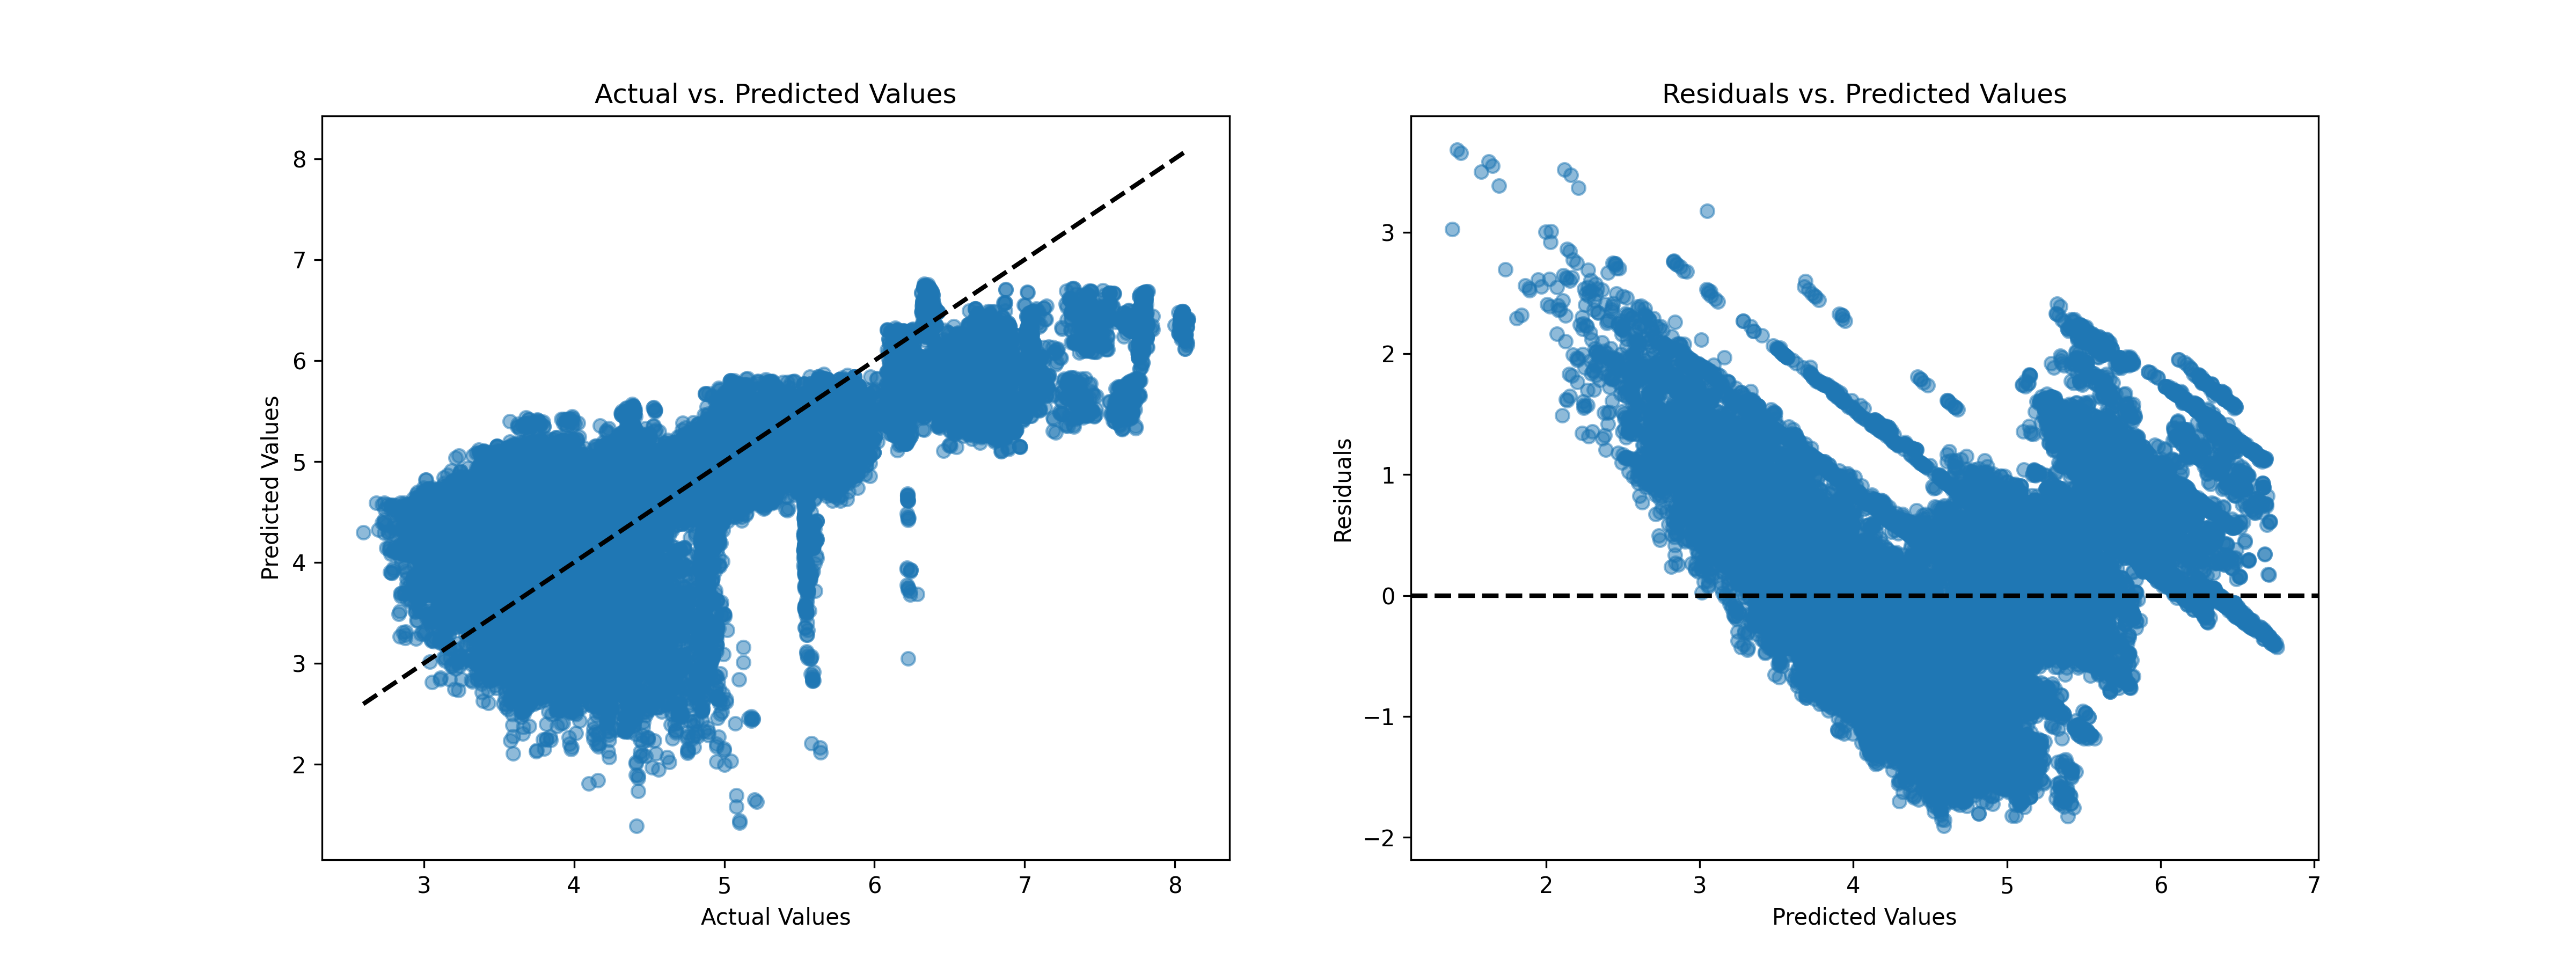
\includegraphics[width=1\textwidth]{../scripts/images/residuals_gpu.png}
    Quelle: Eigene Darstellung, \ref{linreg}.
    \label{pic:residuals}
\end{figure}

\section{Interpretation}

Die Interpretation der Ergebnisse der Modellanalyse bietet wertvolle Einsichten in die Daten 
und das Verhalten des linearen Regressionsmodells. Durch die Verwendung von SHAP-Werten wird 
es möglich, die Beiträge der einzelnen Merkmals zur Vorhersageleistung des Modells nicht nur 
auf globaler Ebene, sondern auch auf lokaler, individueller Ebene zu verstehen. 
Diese tiefgehende Analyse ermöglicht es, das Modell auf seine Fairness, 
Genauigkeit und Transparenz zu überprüfen.


\subsection{Lokale Interpretation}

Die lokale Interpretation konzentriert sich auf das Verständnis der Vorhersagen 
für eine einzelne Beobachtung aus dem Datensatz. Hierzu wird der SHAP Waterfall Plot eingesetzt, 
der eine visuelle Darstellung des Beitrags eines jeden Merkmals zu einer spezifischen Vorhersage liefert.

\begin{figure}[!h]
    \caption{SHAP Waterfall Plot}
    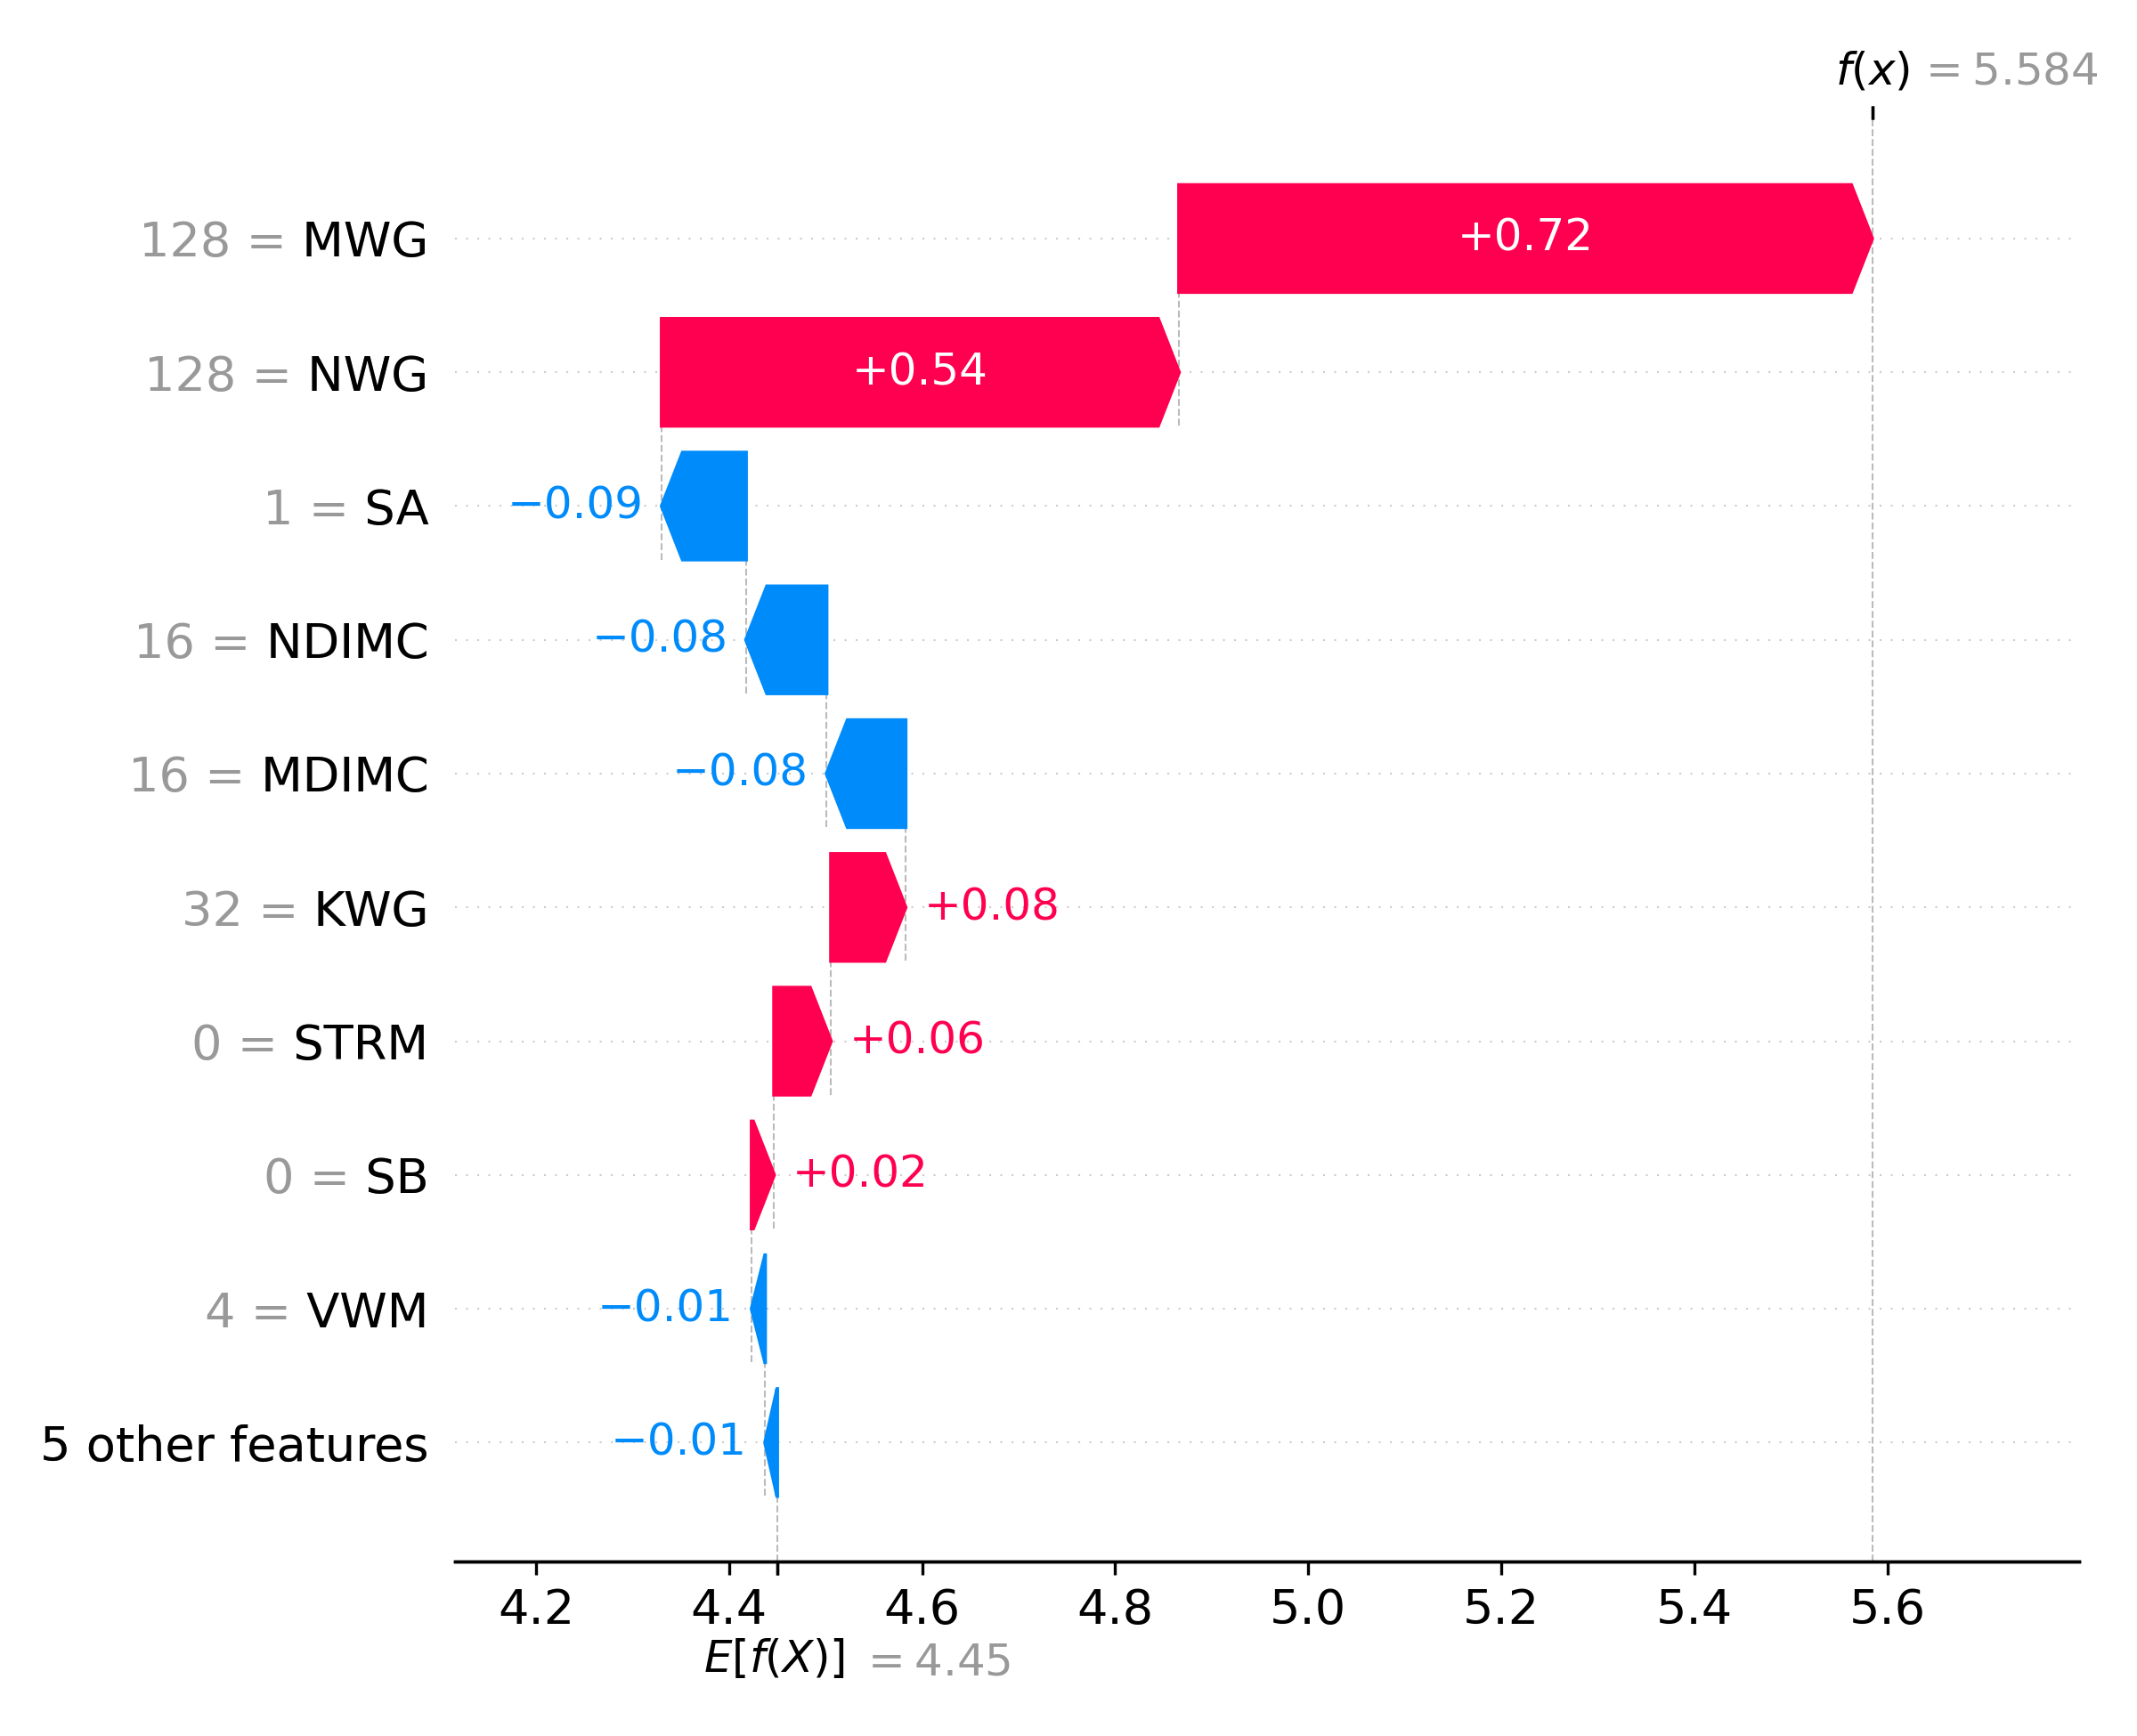
\includegraphics[width=1\textwidth]{../scripts/images/shap_waterfall_plot_gpu.png}
    Quelle: Eigene Darstellung, \ref{linreg}.
    \label{pic:shap_waterfall}
\end{figure}


In Abbildung \ref{pic:shap_waterfall} ist ein Waterfall Plot der ersten Beobachtung $x^{(0)}$ dargestellt, 
der die Zerlegung einer einzelnen Modellvorhersage zeigt. Der Plot beginnt mit dem Basiswert $\mathbb{E}[f(X)] = 4.45$, 
der durchschnittlichen Vorhersage des Modells. 

Von diesem Wert ausgehend, illustrieren die Balken, wie jede Merkmalausprägung – 
angezeigt durch die grauen Zahlen entlang der y-Achse – die Vorhersage $f(x_{j}^{(0)})$ beeinflusst. 
So steigert beispielsweise MWG mit einem Wert von $128$ die Vorhersage deutlich um $+0.72$, 
wohingegen SA mit einem Wert von $1$ die Vorhersage um $-0.09$ verringert.

Rote Balken repräsentieren Merkmals, die die Vorhersage erhöhen, während blaue Balken solche 
darstellen, die sie senken. Die Größe jedes Balkens zeigt das Ausmaß des jeweiligen Beitrags, 
und die abschließende Vorhersage $f(x) = 5.584$ wird am Ende der Kette dieser Effekte erreicht. 

Kleine positive und negative Beiträge von Merkmals wie KWG ($32$), STRM ($0$), SB ($0$) und VWM ($4$) 
zeigen, wie feingranulare Anpassungen der Merkmal-Werte die Vorhersage leicht erhöhen oder senken können.

Für die Beobachtung $x^{(0)}$ führt die kumulative Abweichung der Merkmal-Effekte 
vom Basiswert $\mathbb{E}[f(X)] = 4.45$ zu einem tatsächlichen Modelloutput von $f(x) = 5.584$, 
was eine Differenz von $+1.134$ zwischen der durchschnittlichen Vorhersage 
und der spezifischen Vorhersage für diese Beobachtung offenlegt. 
Diese Differenz entspricht der Summe aller SHAP-Werte für diese konkrete Beobachtung \cite[S. 52f]{Molnar_2023}.

Da die Zielgröße einer logarithmischen Transformation unterzogen wurde, muss diese für die Interpreation wieder rückgängig gemacht werden. 
Dies bedeutet, dass der tatsächliche erwartete Wert der Laufzeit der Exponentialfunktion des prognostizierten Wertes entspricht, also $e^{4.45} \approx 85.63$ ms. 
Dieser Rücktransformationsprozess ist notwendig, um die Modellprognosen in der ursprünglichen Skala der Zielvariablen zu interpretieren.
Dies gilt auch für die konkrete Vorhersage $f(x) = 5.584$. Die prognostizierte Laufzeit für die Beobachtung $x^{(0)}$ beträgt also $e^{5.584} \approx 266.13$ ms.

Dies ermöglicht eine detaillierte Analyse, wie das Modell zu einer bestimmten Vorhersage kommt, 
und hilft dabei, die Beiträge und Interaktionen zwischen verschiedenen Merkmals zu verstehen.

Die lokale Interpretation mittels SHAP-Werten ermöglicht zwar eine präzise Erklärung 
der Modellvorhersagen für individuelle Beobachtungen, jedoch stellt sich bei einer 
solchen Betrachtung das Problem der fehlenden Generalisierbarkeit. 
Lokale Analysen können dazu führen, dass spezifische Merkmal-Kontributionen überinterpretiert werden, 
ohne die übergeordneten Muster und Einflüsse zu berücksichtigen, 
die das Modellverhalten im gesamten Datensatz charakterisieren. 
Eine globale Interpretation ist daher erforderlich, um die Konsistenz und Zuverlässigkeit 
des Modells über verschiedene Beobachtungen hinweg zu erfassen. 

\subsection{Globale Interpretation}

Der folgende Abschnitt widmet sich dieser globalen Sichtweise und untersucht, 
wie die Merkmal-Beiträge sich im Kontext des gesamten Datensatzes darstellen lassen.

\begin{figure}[!h]
    \caption{SHAP Beeswarm Plot}
    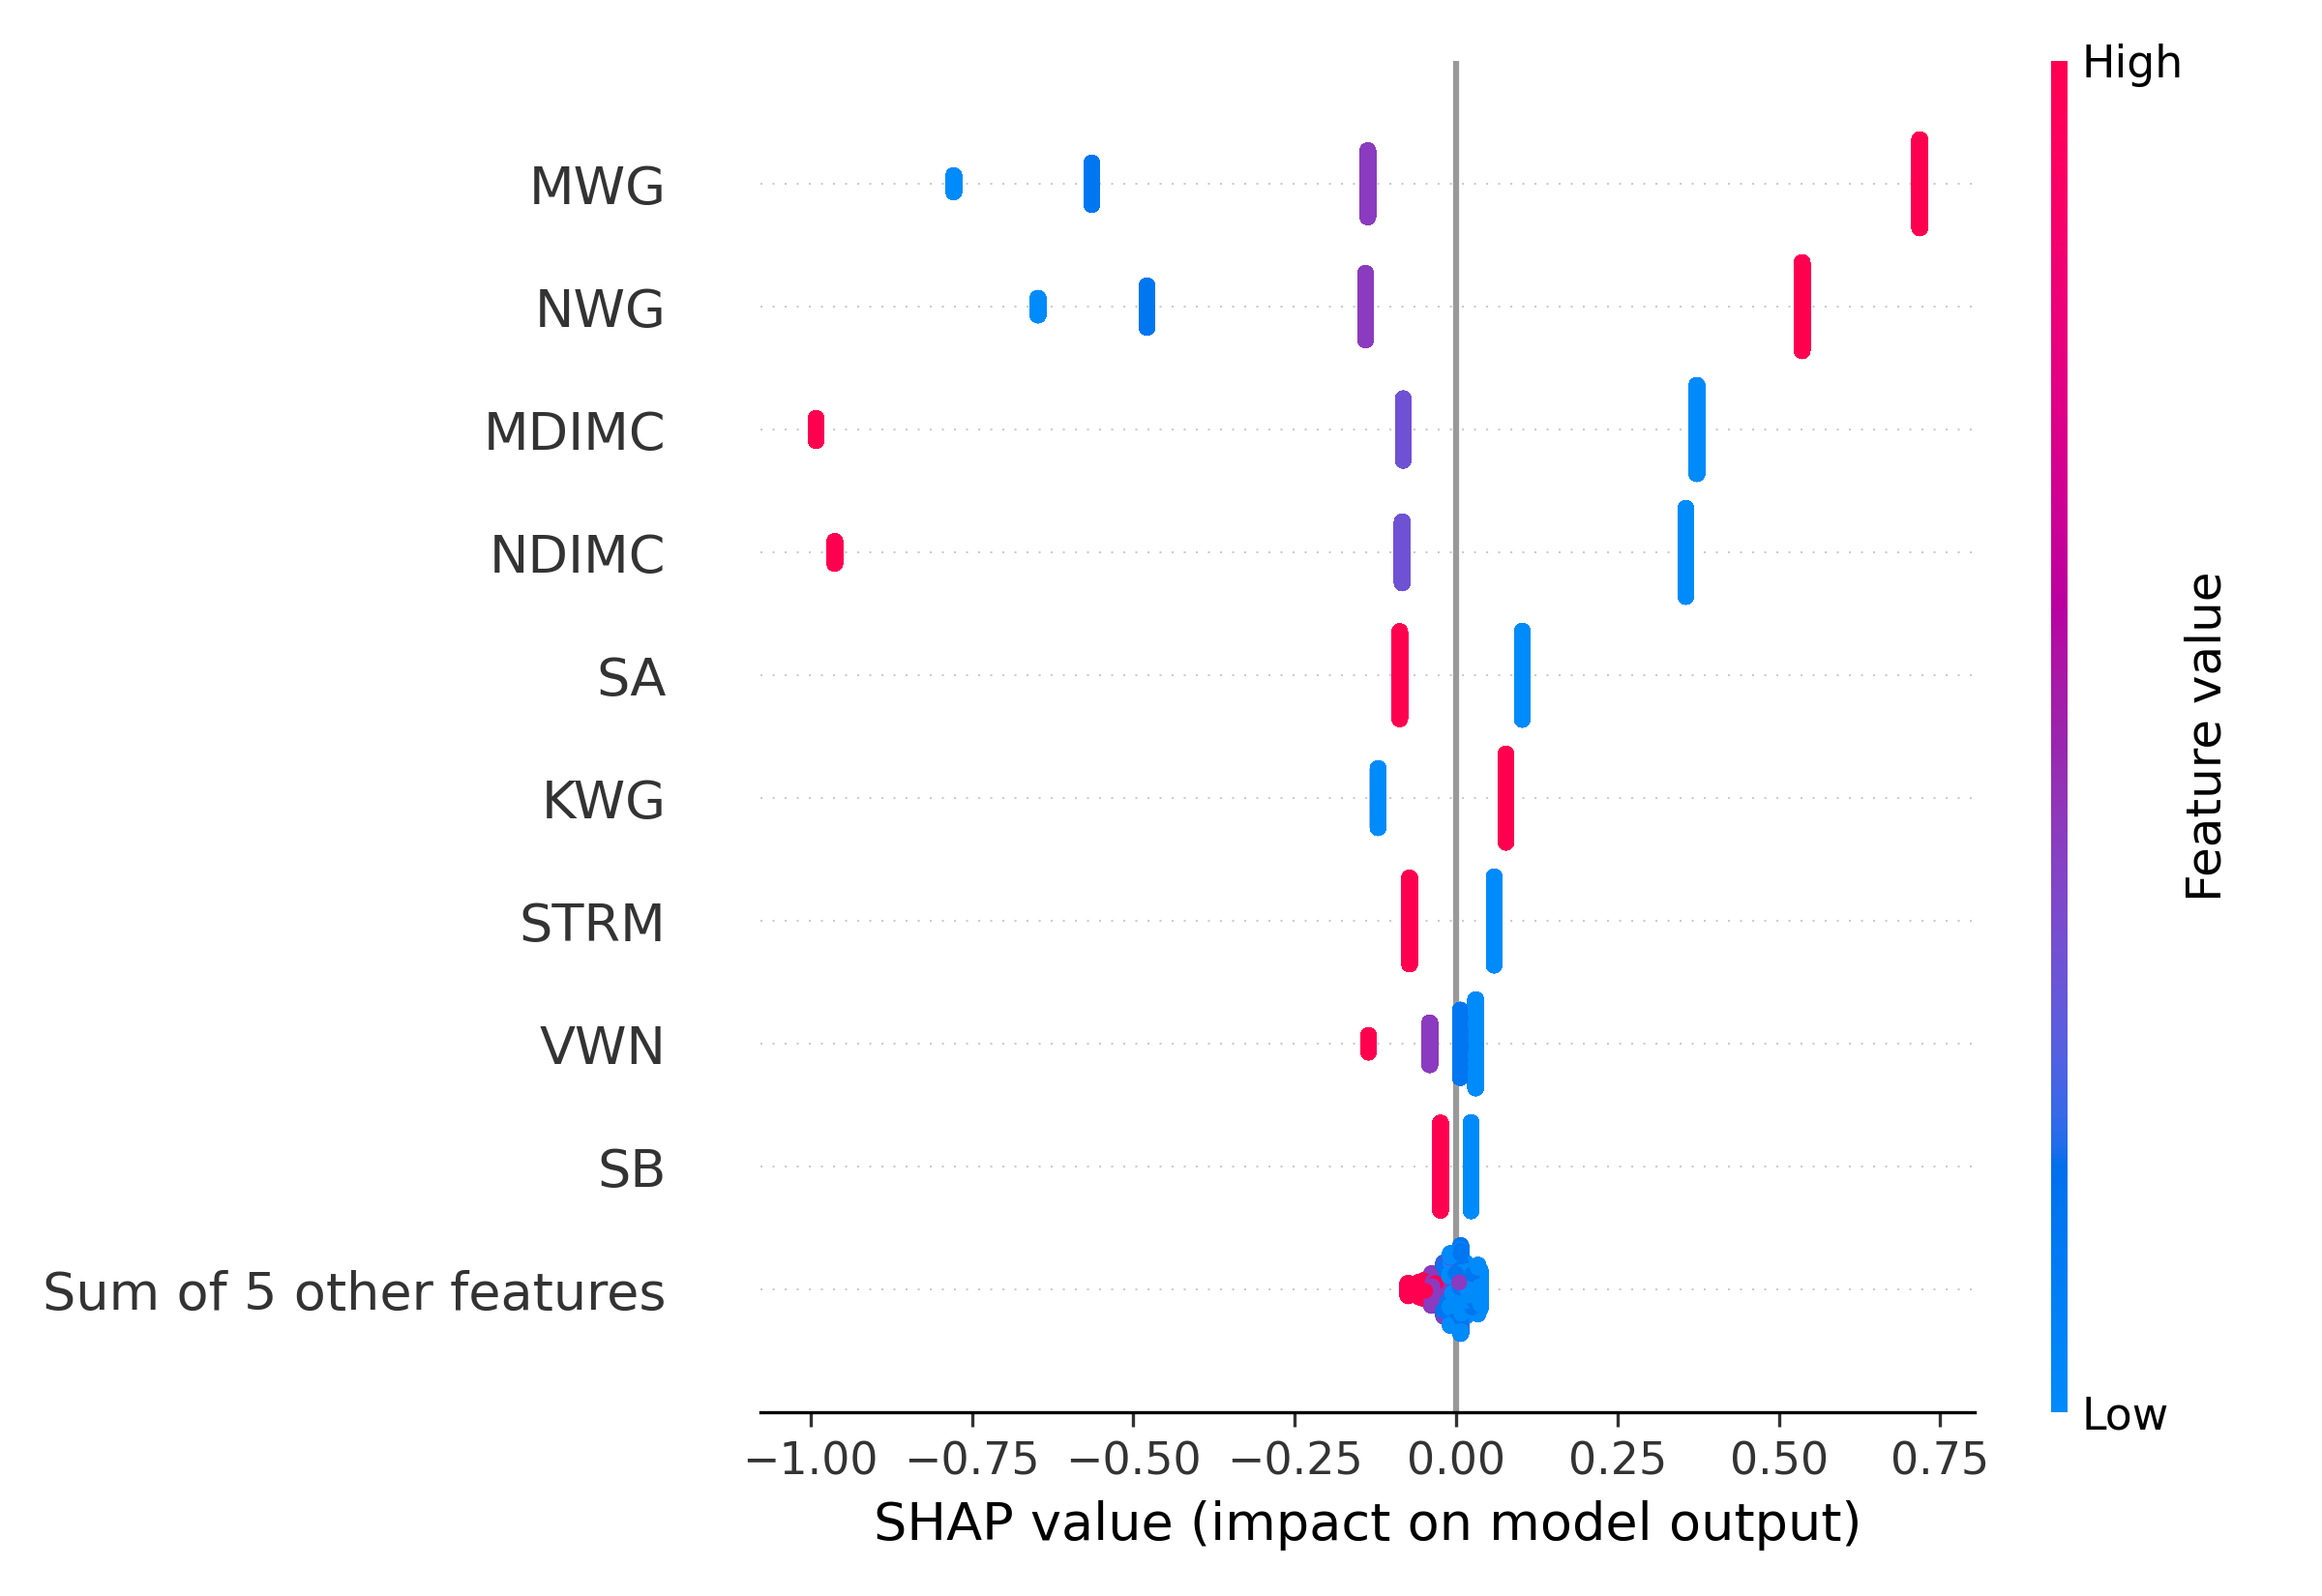
\includegraphics[width=1\textwidth]{../scripts/images/shap_beeswarm_plot_gpu.png}
    Quelle: Eigene Darstellung, \ref{linreg}.
    \label{pic:shap_beeswarm}
\end{figure}

Der SHAP Beeswarm Plot in Abbildung \ref{pic:shap_beeswarm} bietet eine globale 
Sicht auf die Modellvorhersagen, indem er die Verteilung der SHAP-Werte für jedes Merkmal 
über alle Beobachtungen hinweg darstellt. Jeder Punkt repräsentiert eine Beobachtung aus dem Datensatz.
Die Farbe der Punkte zeigt den Merkmals-Wert an: hohe Werte in Rot und niedrige Werte in Blau. 
Die Position auf der x-Achse gibt den Impact des Merkmals auf die Modellvorhersage an. 
Positive SHAP-Werte (rechts von der Nulllinie) zeigen eine Erhöhung der Vorhersage an, 
während negative Werte (links von der Nulllinie) eine Verringerung bedeuten. 

Das Merkmal MWG mit den spezifischen Ausprägungen 16, 32, 64 und 128 zeigt eine Variabilität 
in seinem Einfluss auf die Modellvorhersage. Höhere Werte von MWG, insbesondere 128, 
sind mit einer Zunahme der Vorhersage (positive SHAP-Werte) assoziiert, 
was durch die rechtsseitigen Punkte in der Grafik dargestellt wird. 
iedrigere Werte wie 16 führen hingegen zu einer geringeren Vorhersage, 
erkennbar an den linksseitigen Punkten. Diese Streuung der Punkte zeigt, 
dass die Auswirkung von MWG auf die Vorhersage stark von seiner quantitativen Ausprägung abhängt.

Diese Darstellung ermöglicht es, die Merkmals zu identifizieren, 
die den größten Einfluss auf das Modell haben und wie dieser Einfluss über 
unterschiedliche Beobachtungen variiert.

\begin{figure}[!h]
    \caption{SHAP Bar Plot}
    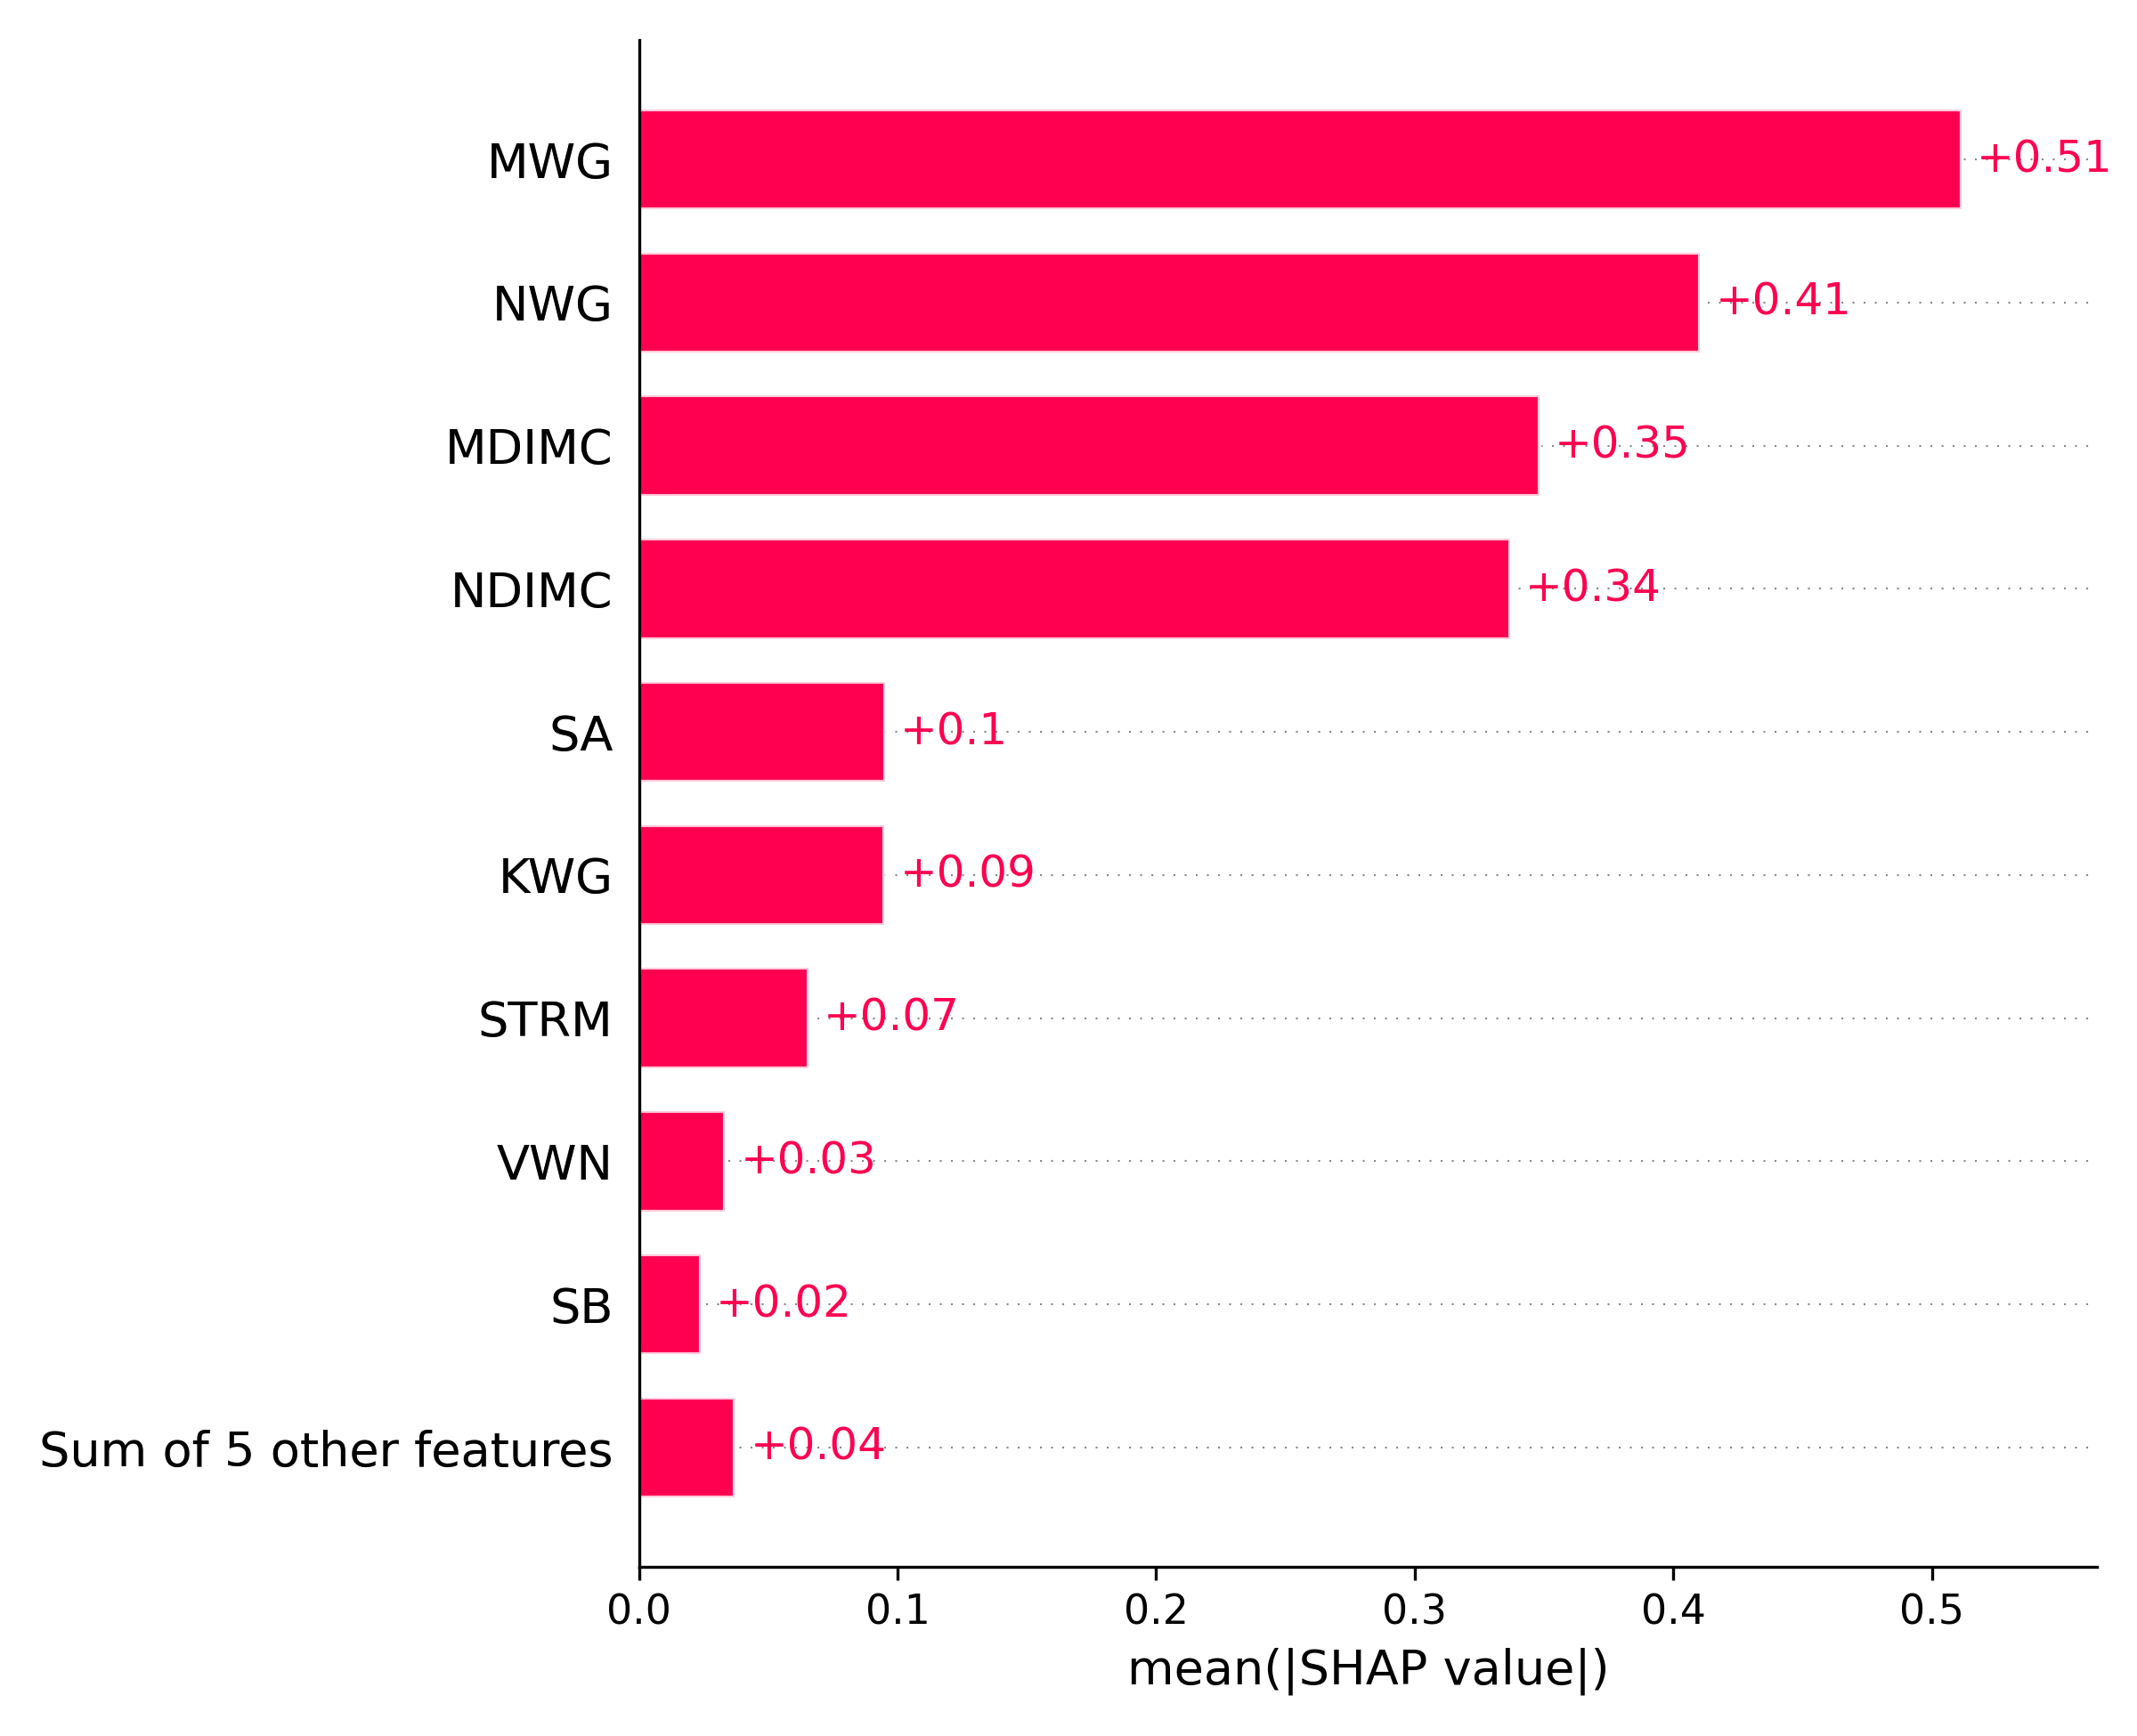
\includegraphics[width=1\textwidth]{../scripts/images/shap_bar_plot_gpu.png}
    Quelle: Eigene Darstellung, \ref{linreg}.
    \label{pic:shap_bar}
\end{figure}

Der SHAP Bar Plot in Abbildung \ref{pic:shap_bar} illustriert die durchschnittliche 
Auswirkung jedes Merkmals auf das Modell, gemessen an der absoluten Größe der SHAP-Werte 
über alle Beobachtungen hinweg. Die Balken zeigen die durchschnittlichen Beiträge der 
Merkmals zur Vorhersage: Je länger der Balken, desto größer ist der Einfluss des jeweiligen Merkmals. 
Hier ist das Merkmal MWG mit dem höchsten durchschnittlichen SHAP-Wert (+0.51) das einflussreichste 
Merkmal, was auf eine starke positive Beziehung zur Zielvariablen hinweist. Die weiteren Merkmals 
folgen in absteigender Reihenfolge ihrer Bedeutung, wobei auch die Summe der Beiträge der 
fünf weiteren Merkmals am unteren Rand der Grafik dargestellt wird.
